\section{RQ2: The $J$ Condition}

\begin{theorem}\label{thm:j}
Assume that the primary's label is correct, that corroborator labels are mutually independent and depend only on the true class (shared or independent), and that selection is uniform with uniform fallback. Let $a = 1-r$ be the probability that a shared tool is a candidate, $b = 1-\varphi$ the probability that an independent tool is a candidate, and $K$ the number of other candidates. Then
\[
P(\text{select a shared tool}) - \frac{s}{n} \;=\; -\,\frac{s(n-s)}{n}\, J\; \E\!\left[\frac{1}{1+K}\right].
\]
\end{theorem}

Both $s(n-s)/n$ and $\E[1/(1+K)]$ are positive, so \emph{the sign of the difference is the sign of $-J$}: provenance beats random iff $J>0$, ties at $J=0$, and loses when $J<0$. \emph{Proof idea:} pair one shared tool with one independent tool; the remaining candidates have the same distribution from the viewpoint of both, so when the two selection probabilities are subtracted every term cancels except $(b-a)\,\E[1/(1+K)]$, and $b-a=J$. If each label is present only with probability $k$, then $a=k(1-r)$ and $b=k(1-\varphi)$, so $b-a=kJ$: \emph{missing labels shrink the effect but never flip its sign}. The closed form matches exact enumeration to $10^{-16}$; a numerical sweep over 2,205 grid points in 5 topologies, checked by independent Monte Carlo, shows no violation.

\paragraph{Example.} In the main topology ($n=3$, $s=1$) with $r=0$ and $\varphi=0.5$ ($J=-0.5$), provenance selects the shared tool with probability $0.583$ versus $0.333$ for random: bad metadata is worse than none.

\paragraph{Preregistered test.} To check that the condition survives the full pipeline (actor, gate, leakage, oracle) and not only the selection formula, we wrote the protocol and hypotheses in advance and ran them on 60 \emph{new} tasks with 5 new seeds, 4 label conditions and 2 policies (4,800 rows, leakage 0.10). One amendment corrected a prediction \emph{before} the run, after a unit test showed that it used a wrong assumption. \Cref{tab:jtest} and \cref{fig:j} show the results. Both main hypotheses (harm when $J<0$, benefit when $J>0$) are supported, and the differences lie close to the predictions. H-J3 (equivalence at $J=0$, margin $\pm0.08$) is \emph{not} confirmed: the 90\% CI $[+0.013,+0.117]$ exceeds the margin. Its power (about 59\%) was not planned, and we do not interpret the result as harm at $J=0$, because the protocol did not register that hypothesis.

\begin{table}[t]
\centering
\caption{Preregistered test of the $J$ condition: unsafe decision rates under the targeted fault (\checkmark{} supported, $\times$ not supported).}
\label{tab:jtest}
\small
\setlength{\tabcolsep}{3.5pt}
\begin{tabular}{lrrrrll}
\toprule
Condition & Prov. & Random & $\Delta$ & Predicted & 95\% CI & Hypothesis \\
\midrule
$J=+0.8$ ($r$ 0.9, $\varphi$ 0.1) & 0.087 & 0.263 & $-0.177$ & $-0.176$ & $[-0.233,-0.120]$ & H-J2 \checkmark \\
$J=0$ ($r$ 0.5, $\varphi$ 0.5) & 0.320 & 0.257 & $+0.063$ & $0.000$ & $[+0.003,+0.127]$ & H-J3 $\times$ \\
$J=-0.5$ ($r$ 0.1, $\varphi$ 0.6) & 0.423 & 0.290 & $+0.133$ & $+0.160$ & $[+0.070,+0.200]$ & H-J1 \checkmark \\
Survey ($r$ 0.57, $\varphi$ 0, $k$ 0.55) & 0.173 & 0.267 & $-0.093$ & $-0.091$ & $[-0.157,-0.033]$ & H-J4 \checkmark \\
\bottomrule
\end{tabular}
\end{table}

\begin{figure}[t]
  \centering
  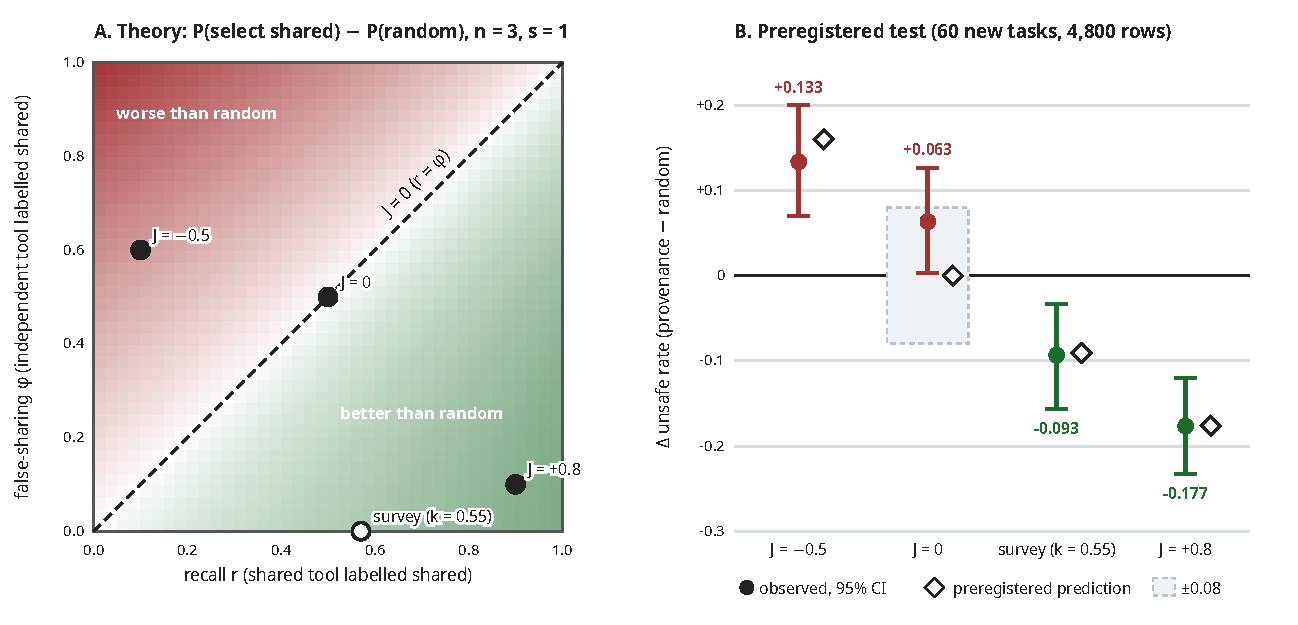
\includegraphics[width=\linewidth]{figures/rq2-j-condition.pdf}
  \caption{(A) Closed-form $P(\text{select shared}) - s/n$ for the main topology over $(r,\varphi)$: green is better than random, red is worse; the boundary is exactly the diagonal $J=0$. The hollow point (survey-calibrated) has missing labels and is shown for reference only. (B) Unsafe-rate differences in the preregistered test with 95\% CIs; diamonds are preregistered predictions; the grey band is the $\pm0.08$ equivalence margin.}
  \label{fig:j}
\end{figure}

\paragraph{Limits of RQ2.} This is a simulation we designed, so the outcome is largely implied by the model; its value lies in test discipline (predictions written in advance, new tasks), not novelty. The theorem does not cover labels correlated across tools, a wrong primary label (which is exactly the robustness-gate model of RQ1), or selection of several corroborators.
